% !TeX document-id = {2870843d-1baa-4f6a-bd0a-a5c796104a32}
% !BIB TS-program = biber
% !TeX encoding = UTF-8
% TU Delft beamer template

\documentclass{beamer}
\usepackage[english]{babel}
\usepackage{csquotes}
\usepackage{calc}
\usepackage[absolute,overlay]{textpos}
\usepackage{graphicx}
\usepackage{subfig}
\usepackage{mathtools}
\usepackage{amsfonts}
\usepackage{amsthm}
\usepackage{comment}
\usepackage{siunitx}
% \usepackage{MnSymbol,wasysym}
\usepackage{array}
\usepackage{emoji}
\usepackage{tikz}
\usepackage{graphicx}

\setemojifont{TwemojiMozilla}

\setbeamertemplate{navigation symbols}{} % remove navigation symbols

\usepackage{caption}
\captionsetup[figure]{labelformat=empty}%

\mode<presentation>{\usetheme[verticalbar=false]{tud}}

% BIB SETTINGS
\usepackage[
    backend=biber,
    giveninits=true,
    maxnames=30,
    maxcitenames=20,
    uniquename=init,
    url=false,
    style=authoryear,
]{biblatex}
\addbibresource{bibfile.bib}
\setlength\bibitemsep{0.3cm} % space between entries in the reference list
\renewcommand{\bibfont}{\normalfont\scriptsize}
\setbeamerfont{footnote}{size=\tiny}
\renewcommand{\cite}[1]{\footnote<.->[frame]{\fullcite{#1}}}
\setlength{\TPHorizModule}{\paperwidth}
\setlength{\TPVertModule}{\paperheight}

\newcommand{\absimage}[4][0.5,0.5]{%
	\begin{textblock}{#3}%width
		[#1]% alignment anchor within image (centered by default)
		(#2)% position on the page (origin is top left)
		\includegraphics[width=#3\paperwidth]{#4}%
\end{textblock}}

\newcommand{\mininomen}[2][1]{{\let\thefootnote\relax%
	\footnotetext{\begin{tabular}{*{#1}{@{\!}>{\centering\arraybackslash}p{1em}@{\;}p{\textwidth/#1-2em}}}%
	#2\end{tabular}}}}

\title{Taller de Git!}
\author{ComCom}
\institute{DC - FCEyN - UBA}

% http://latexcolor.com/
\definecolor{lightseagreen}{rgb}{0.13, 0.7, 0.67}
\definecolor{tangelo}{rgb}{0.98, 0.3, 0.0}
\definecolor{git}{rgb}{0.94, 0.309, 0.2}

\setbeamercolor{structure}{fg=lightseagreen}

\definecolor{x11gray}{rgb}{0.75, 0.75, 0.75}
\newcommand{\code}[1]{\Colorbox{x11gray}{\lstinline{#1}}}

\newenvironment{ejercicio}[1]{
% \setbeamercolor{block title}{bg=tangelo, fg=white}
\begin{exampleblock}{#1}
}{
\end{exampleblock}
}

\newenvironment{resumen}[1]{
\setbeamercolor{block title}{bg=git, fg=white}
\begin{block}{#1}
}{
\end{block}
}

\newenvironment{comando}{
\setbeamercolor{block body}{bg=git, fg=white}
\begin{block}{}
\begin{center}
\LARGE
\begin{texttt}
}{
\end{texttt}
\end{center}
\end{block}
}


\begin{document}
\begin{frame}
  \titlepage
  \begin{figure}[ht]
      \begin{center}
          
\includegraphics[height=1in]{images/logo-taller.png}
      \end{center}
  \end{figure}
\end{frame}

\begin{frame}{La Shell}
\begin{block}{¿Qué es?}
    \begin{itemize}
        \item Interactuamos con la computadora a través de una interfaz.
        \pause
        \item Puede ser gráfica (GUI).
            \begin{figure}
            \begin{minipage}{.5\textwidth}
              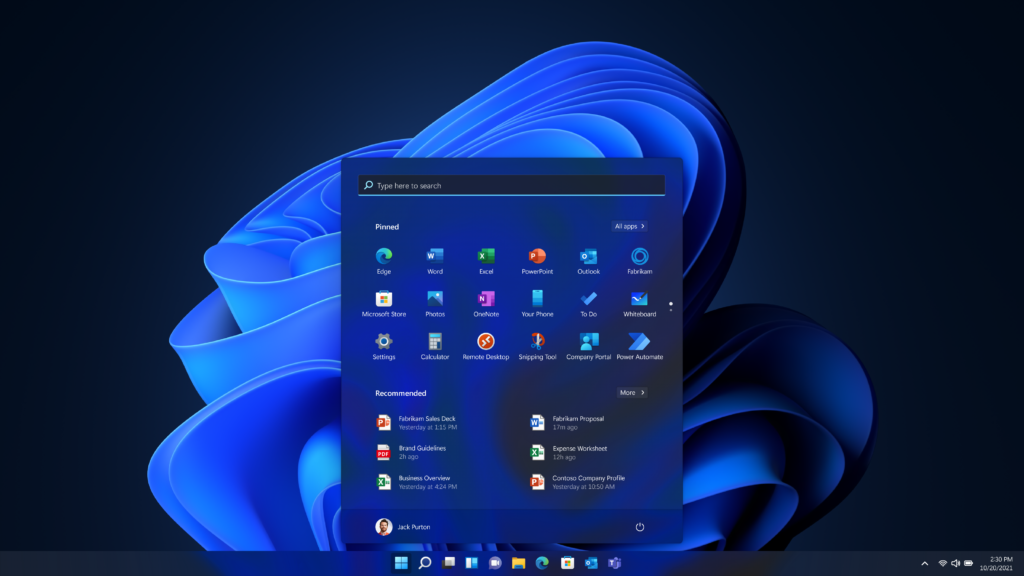
\includegraphics[width=.8\linewidth]{images/windows-gui.png}
            \end{minipage}%
            \begin{minipage}{.5\textwidth}
              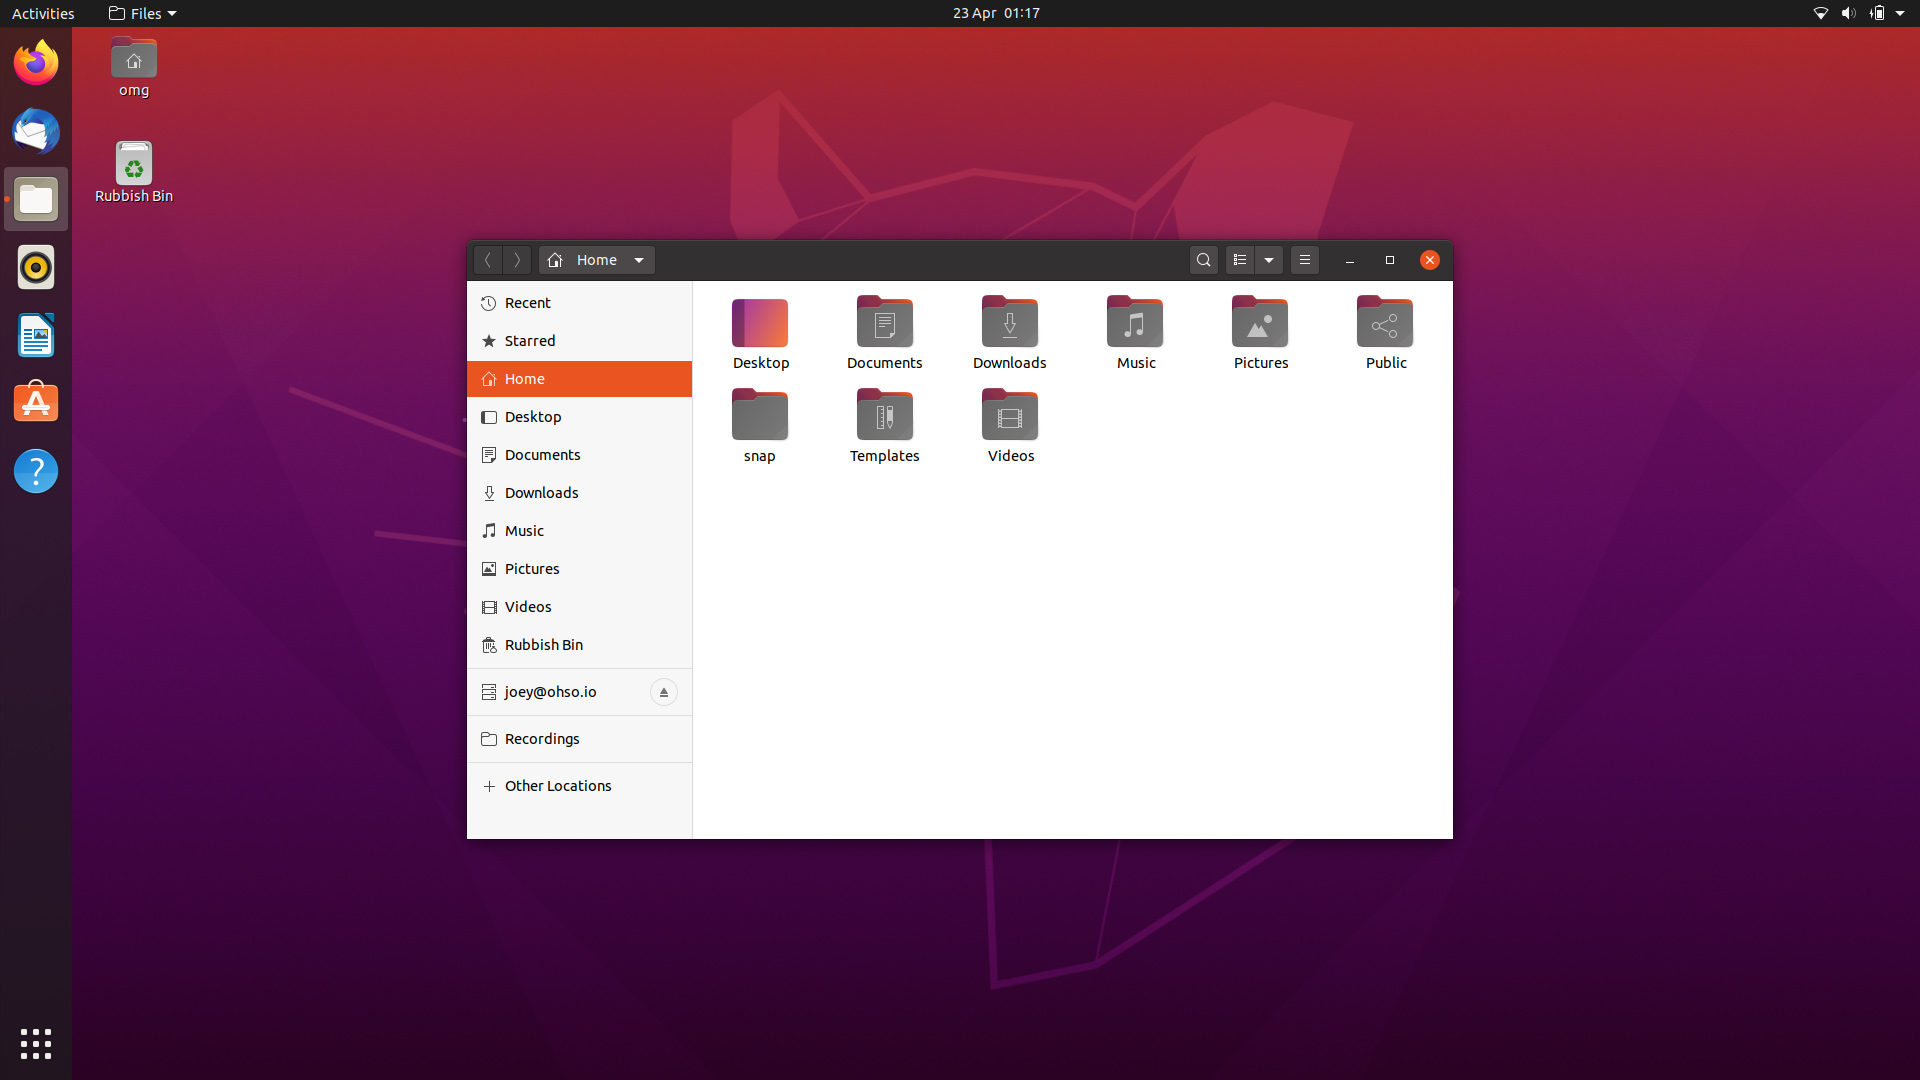
\includegraphics[width=.8\linewidth]{images/ubuntu-gui.jpg}
            \end{minipage}
            \end{figure}
        \pause
        \item O de línea de comando (CLI).
    \end{itemize}
\end{block}

\end{frame}

\begin{frame}{La Shell (2)}
    \begin{block}{¿Qué es? (2)}
        \begin{itemize}
                \item Bash \hookrightarrow\ \textit{Bourne-Again SHell}
            \pause
            \item Para abrir un \textit{shell prompt,} necesitamos una terminal.
            \pause
        \end{itemize}
    \begin{centering}
    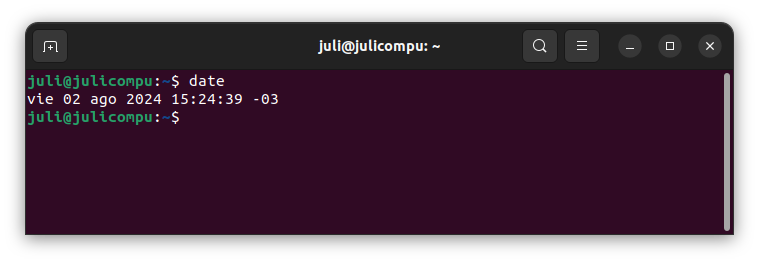
\includegraphics[height=1.5in]{images/bash-1.png}        
    \end{centering}
    \end{block}

\end{frame}

\begin{frame}{La Shell (3)}
% But how does the shell know how to find the date or echo programs? Well, the shell is a programming environment, just like Python or Ruby, and so it has variables, conditionals, loops, and functions (next lecture!). When you run commands in your shell, you are really writing a small bit of code that your shell interprets. If the shell is asked to execute a command that doesn’t match one of its programming keywords, it consults an environment variable called $PATH that lists which directories the shell should search for programs when it is given a command:
    \begin{block}{¿Cómo se usa?}
        \centering
        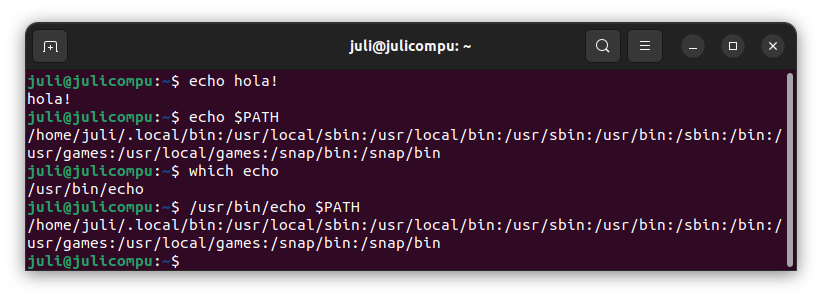
\includegraphics[width=4.5in]{images/bash-2.png}
    \end{block}
    
\end{frame}

\begin{frame}{La Shell (4)}
\begin{block}{Navegando la Shell}
        \vspace{-0.3cm}
        \centering
        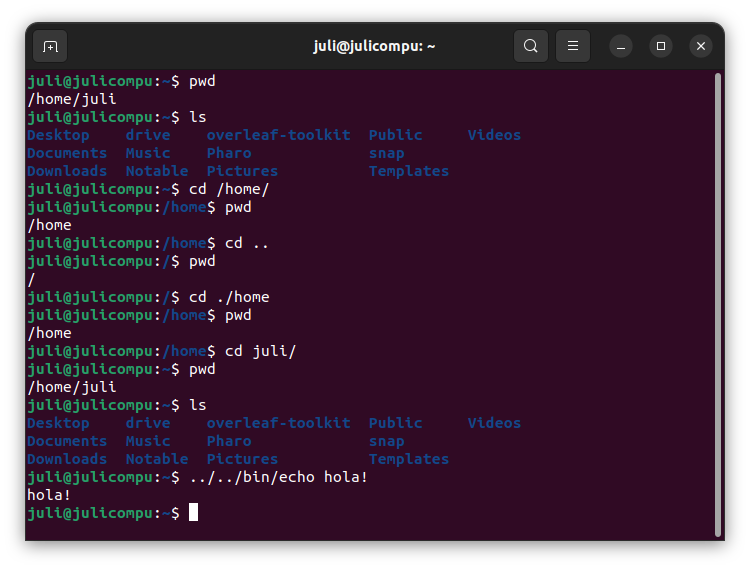
\includegraphics[width=4in]{images/bash-3.png}
\end{block}
\end{frame}

\begin{frame}{La Shell (5)}
\begin{block}{Conectando programas}
        \centering
        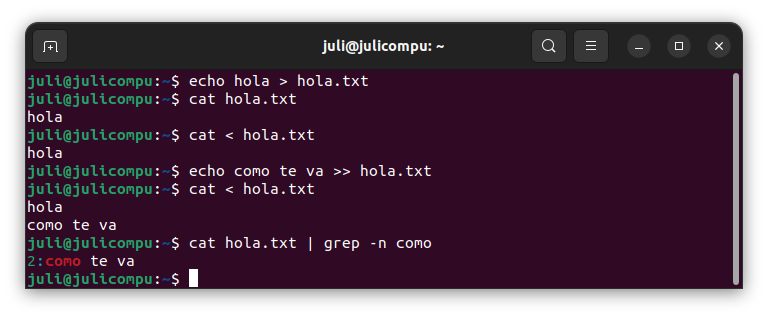
\includegraphics[width=4in]{images/bash-4.png}
\end{block}
\end{frame}

\end{document}